\documentclass[tikz, border=10pt]{standalone}
\usepackage{tikz}
\usepackage{xcolor}

\usetikzlibrary{shapes, arrows, positioning, fit, calc}

% Define colors
\definecolor{UCMBlue}{RGB}{4, 171, 226}
\definecolor{FixedBlue}{RGB}{20, 65, 134}
\definecolor{AdaptRed}{RGB}{200, 40, 40}
\definecolor{AccentGreen}{RGB}{0, 130, 100}
\definecolor{LightGray}{RGB}{240, 240, 240}

% Define styles
\tikzstyle{conv} = [
	draw=FixedBlue,
	fill=FixedBlue!20,
	thick,
	rounded corners=2pt,
	minimum width=1.4cm,
	minimum height=0.8cm,
	font=\tiny,
	align=center
]

\tikzstyle{deconv} = [
	draw=AdaptRed,
	fill=AdaptRed!20,
	thick,
	rounded corners=2pt,
	minimum width=1.4cm,
	minimum height=0.8cm,
	font=\tiny,
	align=center
]

\tikzstyle{upconv} = [
	draw=AdaptRed,
	fill=AdaptRed!10,
	thick,
	rounded corners=2pt,
	minimum width=1.4cm,
	minimum height=0.8cm,
	font=\tiny,
	align=center
]

\tikzstyle{bottle} = [
	draw=AccentGreen,
	fill=AccentGreen!20,
	thick,
	rounded corners=2pt,
	minimum width=1.4cm,
	minimum height=0.8cm,
	font=\tiny,
	align=center
]

\tikzstyle{data} = [
	draw=gray,
	fill=LightGray,
	thick,
	minimum width=0.9cm,
	minimum height=0.7cm,
	font=\tiny,
	align=center
]

\tikzstyle{arrow} = [thick, ->, >=stealth]
\tikzstyle{pool} = [thick, ->, >=stealth, draw=AccentGreen]
\tikzstyle{up} = [thick, ->, >=stealth, draw=AdaptRed]
\tikzstyle{copy} = [line width=2pt, ->, >=stealth, draw=gray!60]

\begin{document}

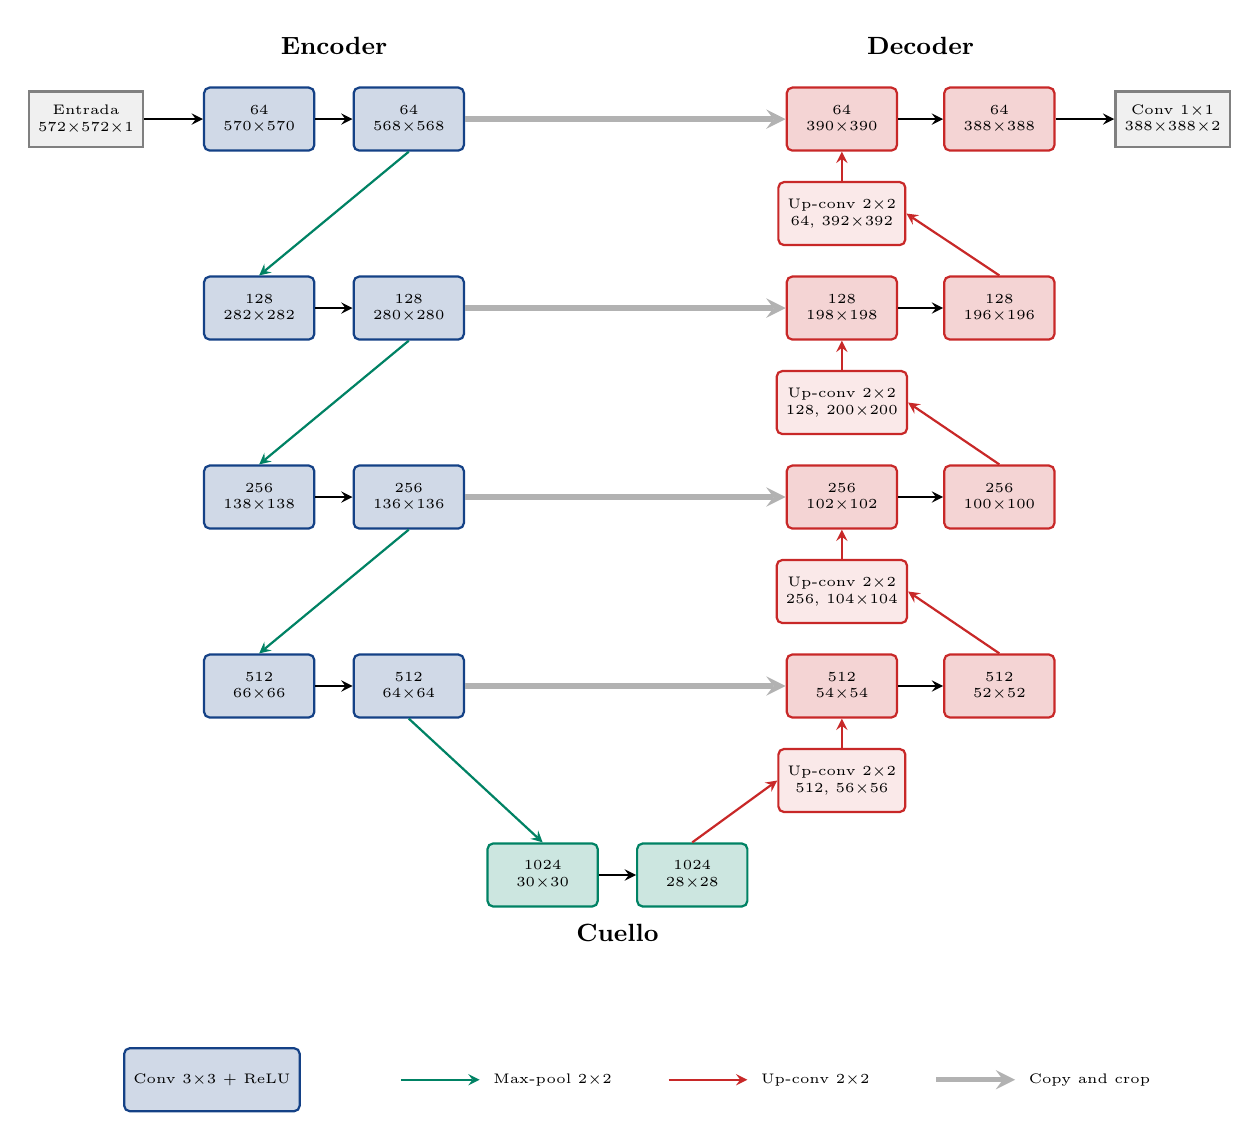
\begin{tikzpicture}[node distance=0.8cm]

	% ========== INPUT ==========
	\node[data] (in) at (-2.2, 9.6) {Entrada\\ $572{\times}572{\times}1$};

	% ========== ENCODER (izquierda) ==========
	% Nivel 1: 64 canales
	\node[conv] (e1a) at (0, 9.6) {64\\ $570{\times}570$};
	\node[conv] (e1b) at (1.9, 9.6) {64\\ $568{\times}568$};

	% Nivel 2: 128 canales
	\node[conv] (e2a) at (0, 7.2) {128\\ $282{\times}282$};
	\node[conv] (e2b) at (1.9, 7.2) {128\\ $280{\times}280$};

	% Nivel 3: 256 canales
	\node[conv] (e3a) at (0, 4.8) {256\\ $138{\times}138$};
	\node[conv] (e3b) at (1.9, 4.8) {256\\ $136{\times}136$};

	% Nivel 4: 512 canales
	\node[conv] (e4a) at (0, 2.4) {512\\ $66{\times}66$};
	\node[conv] (e4b) at (1.9, 2.4) {512\\ $64{\times}64$};

	% ========== CUELLO DE BOTELLA ==========
	\node[bottle] (ba) at (3.6, 0) {1024\\ $30{\times}30$};
	\node[bottle] (bb) at (5.5, 0) {1024\\ $28{\times}28$};

	% ========== DECODER (derecha) ==========
	% Nivel 4: up-conv + 2 convs
	\node[upconv] (u4) at (7.4, 1.2) {Up-conv 2$\times$2\\ $512$, $56{\times}56$};
	\node[deconv] (d4a) at (7.4, 2.4) {512\\ $54{\times}54$};
	\node[deconv] (d4b) at (9.4, 2.4) {512\\ $52{\times}52$};

	% Nivel 3
	\node[upconv] (u3) at (7.4, 3.6) {Up-conv 2$\times$2\\ $256$, $104{\times}104$};
	\node[deconv] (d3a) at (7.4, 4.8) {256\\ $102{\times}102$};
	\node[deconv] (d3b) at (9.4, 4.8) {256\\ $100{\times}100$};

	% Nivel 2
	\node[upconv] (u2) at (7.4, 6.0) {Up-conv 2$\times$2\\ $128$, $200{\times}200$};
	\node[deconv] (d2a) at (7.4, 7.2) {128\\ $198{\times}198$};
	\node[deconv] (d2b) at (9.4, 7.2) {128\\ $196{\times}196$};

	% Nivel 1
	\node[upconv] (u1) at (7.4, 8.4) {Up-conv 2$\times$2\\ $64$, $392{\times}392$};
	\node[deconv] (d1a) at (7.4, 9.6) {64\\ $390{\times}390$};
	\node[deconv] (d1b) at (9.4, 9.6) {64\\ $388{\times}388$};

	% Salida
	\node[data] (out) at (11.6, 9.6) {Conv $1{\times}1$\\ $388{\times}388{\times}2$};

	% ========== CONEXIONES: ENCODER ==========
	\draw[arrow] (in.east) -- (e1a.west);
	\draw[arrow] (e1a.east) -- (e1b.west);
	\draw[arrow] (e2a.east) -- (e2b.west);
	\draw[arrow] (e3a.east) -- (e3b.west);
	\draw[arrow] (e4a.east) -- (e4b.west);

	% Max-pool 2x2 (de b_i a a_{i+1})
	\draw[pool] (e1b.south) -- (e2a.north);
	\draw[pool] (e2b.south) -- (e3a.north);
	\draw[pool] (e3b.south) -- (e4a.north);
	\draw[pool] (e4b.south) -- (ba.north);

	% ========== CONEXIONES: CUELLO ==========
	\draw[arrow] (ba.east) -- (bb.west);

	% ========== CONEXIONES: DECODER ==========
	% Up-conv desde la salida del nivel inferior
	\draw[up] (bb.north) -- (u4.west);
	\draw[up] (d4b.north) -- (u3.east);
	\draw[up] (d3b.north) -- (u2.east);
	\draw[up] (d2b.north) -- (u1.east);

	% Up-conv -> primera convolucion del nivel (tras concatenar)
	\draw[up] (u4.north) -- (d4a.south);
	\draw[up] (u3.north) -- (d3a.south);
	\draw[up] (u2.north) -- (d2a.south);
	\draw[up] (u1.north) -- (d1a.south);

	% Dos convoluciones 3x3 por nivel
	\draw[arrow] (d4a.east) -- (d4b.west);
	\draw[arrow] (d3a.east) -- (d3b.west);
	\draw[arrow] (d2a.east) -- (d2b.west);
	\draw[arrow] (d1a.east) -- (d1b.west);

	\draw[arrow] (d1b.east) -- (out.west);

	% ========== COPY AND CROP ==========
	\draw[copy] (e1b.east) -- (d1a.west);
	\draw[copy] (e2b.east) -- (d2a.west);
	\draw[copy] (e3b.east) -- (d3a.west);
	\draw[copy] (e4b.east) -- (d4a.west);

	% ========== ETIQUETAS ==========
	\node[font=\small, anchor=south] at (0.95, 10.3) {\textbf{Encoder}};
	\node[font=\small, anchor=south] at (8.4, 10.3) {\textbf{Decoder}};
	\node[font=\small, anchor=north] at (4.55, -0.5) {\textbf{Cuello}};

	% ========== LEYENDA ==========
	\node[conv, minimum width=1.9cm, font=\tiny] at (-0.6, -2.6) {Conv $3{\times}3$ + ReLU};
	\draw[pool] (1.8, -2.6) -- (2.8, -2.6);
	\node[font=\tiny, anchor=west] at (2.85, -2.6) {Max-pool $2{\times}2$};
	\draw[up] (5.2, -2.6) -- (6.2, -2.6);
	\node[font=\tiny, anchor=west] at (6.25, -2.6) {Up-conv $2{\times}2$};
	\draw[copy] (8.6, -2.6) -- (9.6, -2.6);
	\node[font=\tiny, anchor=west] at (9.65, -2.6) {Copy and crop};

\end{tikzpicture}

\end{document}
